\begin{figure}
  \setlength{\unitlength}{\textwidth}
\fbox{
        \begin{picture}(1,0.5)(0,0.255)

      % % % Parkinson Data 
      \put(0.025,0.5){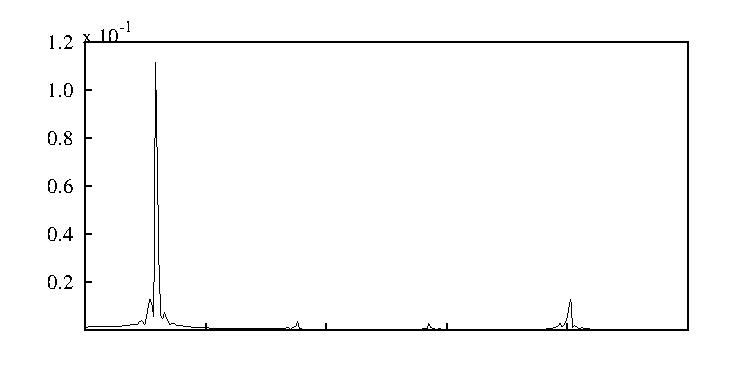
\includegraphics[width=0.5\unitlength]{../FnP/gnuplot/spectrum_pi1_10_pi2_0.eps}}
      \put(0.5,0.5){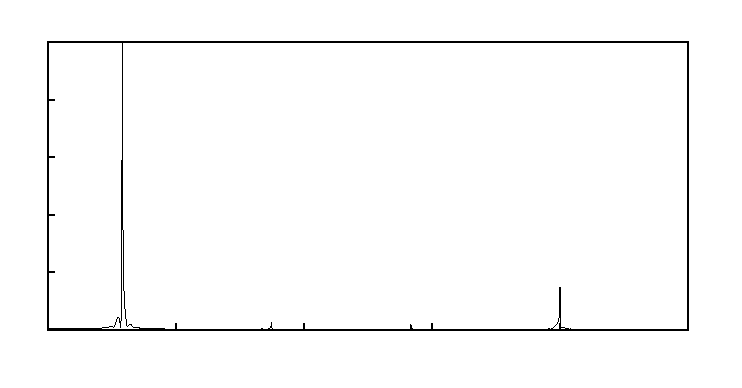
\includegraphics[width=0.5\unitlength]{../FnP/gnuplot/spectrum_pi1_10_pi2_0_3.eps}}
      \put(0.025,0.27){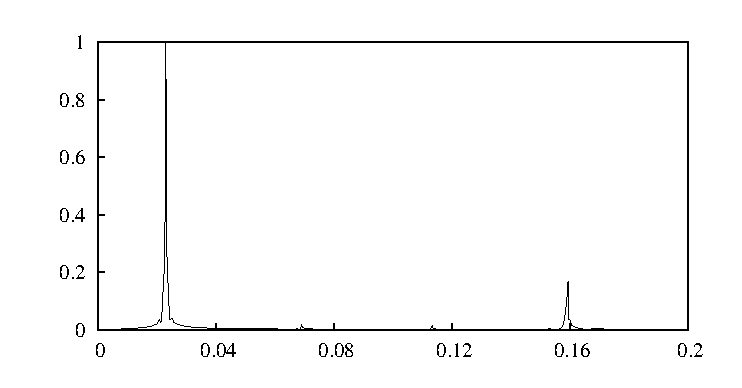
\includegraphics[width=0.5\unitlength]{../FnP/gnuplot/spectrum_pi1_10_pi2_0_54.eps}}
      \put(0.5,0.27){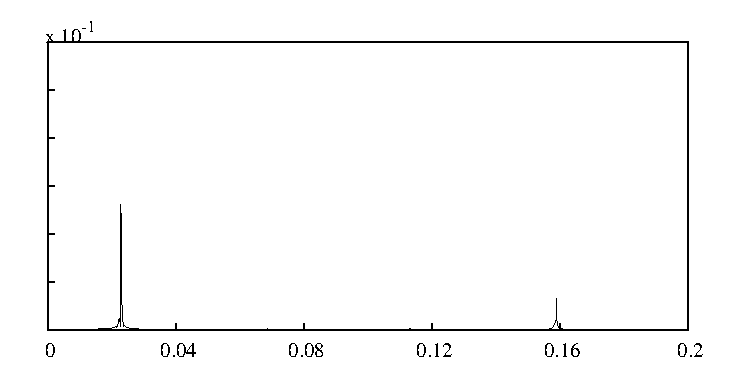
\includegraphics[width=0.5\unitlength]{../FnP/gnuplot/spectrum_pi1_10_pi2_0_7.eps}}
      



      
      \put(0.47,0.709){\small(a)}
      \put(0.94,0.709){\small(b)}
      \put(0.47,0.475){\small(c)}
      \put(0.94,0.475){\small(d)}

      
    \end{picture}
}
  \caption{Power spectrum of velocity at four different damping levels where (a) \massdamp$=0$, (b) \massdamp$=0$, (c) \massdamp$=0$ and (d) \massdamp$=0$ at \massstiff $=10$ (\ustar$=40$). The two peaks present in the plots represent the galloping signal and the shedding signal where the galloping signal is represented by the large peak. The galloping tends to get weaker as \massdamp \ is increased while shedding remains constant}
    \label{fig:spectrum_pi1_10}
\end{figure}

 %vspace{10cm}
